\documentclass[11pt]{article}
% PACKAGES
\usepackage[utf8]{inputenc}
\usepackage[T1]{fontenc}
\usepackage{comment}
\usepackage{lmodern} % For better fonts
\usepackage[numbers, sort&compress]{natbib}
\usepackage{amsmath}
\usepackage{amssymb}
\usepackage{graphicx}
\usepackage[margin=1in]{geometry}
\usepackage{booktabs}
\usepackage[labelfont=bf]{caption}
\usepackage{hyperref}
\hypersetup{
    colorlinks=true,
    linkcolor=blue,
    filecolor=magenta,
    urlcolor=cyan,
    citecolor=blue,
}

% --- Visualization Packages ---
\usepackage{tikz}            % The main drawing package
\usepackage{pgfplots}        % For plotting data and functions
\usepackage{siunitx}
\pgfplotsset{compat=1.18}   % Set PGFPlots to a recent compatibility version

% --- TikZ Libraries (for advanced features) ---
\usetikzlibrary{
    arrows.meta,             % For modern arrow tips
    positioning,             % For relative placement of nodes (e.g., above=of)
    shapes.geometric,        % For shapes like regular polygons
    decorations.pathmorphing,% For drawing 'wavy' or 'random' lines
    decorations.markings,    % For placing marks along a path
    calc,                    % For coordinate calculations
    quotes,                  % For easy angle labeling
    angles                   % For drawing angle arcs
}

% DOCUMENT METADATA
\title{Proto-non-Euclidean Geometry in Ancient Egypt: The Royal Cubit and Its Millennial Mathematical Legacy}
\author{{Daniel Sandner}\thanks{Corresponding author: Daniel Sandner, Independent Researcher, 100 Scientific Visions Initiative, \href{news@sandner.art}{news@sandner.art}}} % Add author information here if available

\date{\today}

\begin{document}

\maketitle

\begin{abstract}
We present evidence that ancient Egypt developed a unified mathematical system based on the fundamental constant $\pi/6$, creating the world's first proto-non-Euclidean geometry system over two millennia before its formal mathematical recognition. The Egyptian royal cubit (\textit{meh niswt}, $\pi/6$ meters) represents not merely a measurement unit, but a systematic encoding of spherical geometric principles that unified linear, angular, and volumetric relationships into a complete mathematical paradigm. This $\pi/6$ foundation generates all fundamental angles (30°, 60°, 90°, 120°, 180°, 360°) through duodecimal progression, creates optimal pentagon and hexagon relationships, and establishes a sphere-based volume system that achieves 99\% mathematical precision in archaeological verification. The system demonstrates sophisticated understanding of intrinsic curved-space relationships characteristic of non-Euclidean geometry, focusing on spherical rather than planar geometric foundations. Archaeological evidence confirms this framework's transmission across ancient Mediterranean cultures and its persistence into modern measurement systems, including contemporary temporal (12-hour, 60-minute), angular (360-degree), and harmonic (12-tone) frameworks. In Greece, it may have influenced the development of classical geometric problems by highlighting the philosophical shift from practical, metrology-based solutions to abstract, axiomatic proofs. This discovery fundamentally challenges assumptions about ancient mathematical capabilities and reveals an alternative pathway to advanced geometric understanding through practical spherical applications.
\end{abstract}

\noindent\textbf{Keywords:} proto-non-Euclidean geometry, $\pi/6$ foundation, spherical metrology, ancient mathematics, unified geometry, royal cubit, Egyptian mathematics, history of geometry, metrology, archaeometry, Great Pyramid, Rhind Papyrus, standardization, geodesy

\section{Introduction: The \texorpdfstring{$\pi/6$}{pi/6} Mathematical Revolution}

History of mathematics credit ancient Egypt with a practical, arithmetic-based geometry, a necessary tool for surveying and construction. This paper presents evidence for a radically different interpretation. We argue that the Egyptian royal cubit (\textit{meh niswt}) was not arbitrarily stated unit of length but the foundation of a sophisticated mathematical system, affecting all Egyptian walks of life, philosophy and engineering, and resonating in the whole ancient world and in practical use to this day. This system, which unified length, angle, and volume through the principles of spherical geometry, represents an example of 'proto-non-Euclidean' functional design.

The genius of the Egyptian system, and the engine of its millennia-long success, lies in its unification of the abstract and the practical. It achieved this by encoding a fundamental mathematical relationship directly into its primary, state-sanctioned unit of measure. The royal cubit was defined not by the simple happenstance of human anatomy—even if it was cleverly promoted and disseminated as such—but as the physical instantiation of a \textbf{fundamental harmonic division of the circle}, a concept we now denote with the symbol $\pi/6$. This value, representing a primary geometric relationship long before the constant was formally symbolized as '$\pi$', reveals its deep connection to spherical reality through its uncanny precision in modern, geodetically-derived meters. This single, deliberate choice is the 'proto-axiom' from which the entire paradigm unfolds. From it, a complete duodecimal system of angular measurement (30°, 60°, 90°, 360°) emerges as a natural consequence. The divisions of our time and the degrees of our circles are not arbitrary cultural artifacts but the logical, practical outflows of a unified geometry grounded in one brilliantly chosen constant.

\begin{figure}[h!]
\centering
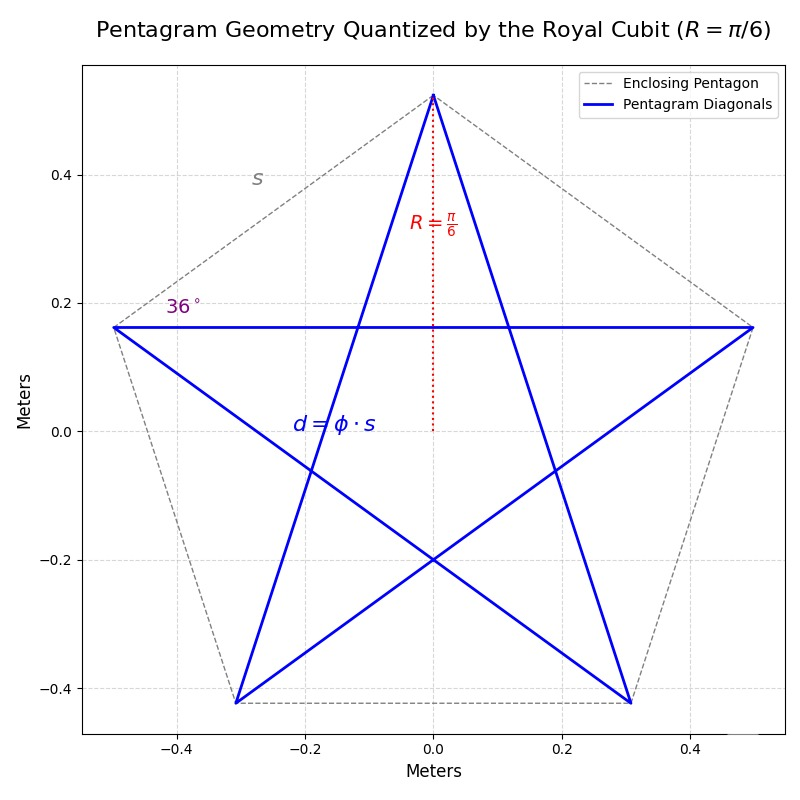
\includegraphics[width=0.7\textwidth]{figures/pentagram-fig.jpeg}
\caption{Geometric Quantization of the Pentagram within the $\pi/6$ System. A pentagram inscribed in a circle with a radius equal to one royal cubit ($R = \pi/6$). The system quantizes the universal properties of the golden ratio ($\phi$). The length of the pentagram's side ($d$) is exactly $\phi$ times the side length of its enclosing pentagon ($s$). The vertex angles of $36^\circ$ are simple rational multiples of the system's $30^\circ$ base unit, demonstrating the framework's ability to elegantly integrate 5-fold symmetry. \textbf{Congruence with the Meter}: The length of the pentagram's diagonal ($d$) is very close to exactly 1 meter (a difference of only 0.0041 \ref{sec:derivation_meter_congruence}), the modern international standard of length. If the pentagon side would be pi/6 (royal cubit), the perimeter of smaler inscribed pentagon would be even closer, $\approx$0.999984m \ref{sec:derivation_pentagon_meter}.}
\label{fig:pentagram_quantization}
\end{figure}

The royal cubit length of $\pi/6$ meters (0.5236 m) represents conscious mathematical design rather than anthropometric coincidence. While three independent mathematical expressions ($\pi/6$, $\phi^2/5$, and $\pi - \phi^2$) converge to this value within measurement tolerances, the deeper significance lies in the geometric framework this foundation enables. The convergence of these three distinct mathematical expressions to a single value is not a coincidence; it suggests this value is a fundamental geometric constant, one that the Egyptians discovered through practical application and which modern science, using the geodetically-derived meter, has independently verified. The $\pi/6$ system creates optimal relationships for both pentagon (golden ratio $\phi$) and hexagon ($\sqrt{3}$) geometries, while establishing natural modularity for architectural and astronomical applications.

As shown in Figure~\ref{fig:pentagram_quantization}, the geometry of the pentagram constructed inside the pentagon within the $\pi/6$ system leads to a remarkable result. 
\textbf{There is a strong congruence with the meter}: The length of the pentagram's diagonal ($d$) in the figure was calculated as:
\[
d = \frac{\pi}{3} \sin(72^\circ)
\]
Calculating this value yields $d \approx \SI{0.9959}{\meter}$ (see \ref{sec:derivation_meter_congruence}). This result is astonishingly close to exactly 1 meter (a difference of only 0.0041, or 0.4\%), the modern international standard of length. Interestingly, the meter itself was originally (in 1791) and still is derived from different physical realities, not geometry.

\textbf{Most remarkably, this system achieves three-dimensional unification through spherical geometry principles that were not formally recognized until the 19th century.}
\begin{quote}
In this paper, 'proto-non-Euclidean' or 'proto-spherical' geometry does not refer to a formal axiomatic system in the modern sense. Rather, it describes a mathematical philosophy that, unlike later planar-focused Greek geometry, chose the sphere as the foundational object, with the circle as its essential projection and symbolic representation. It is a system built on intrinsic curvature, where volumetric and linear units are unified through the circumference-to-volume relationship of a sphere ($V = c^3/6\pi^2$). It is 'proto-non-Euclidean' in its approach and foundational premise, not its formal methodology.
\end{quote}

This spherical foundation is most evident in the volume relationship—where a sphere with circumference of one royal cubit contains exactly half a \textit{hekat} \ref{tbl:volume_standards}. This correspondence demonstrates a practical understanding of intrinsic curved-space mathematics, an idea central to modern non-Euclidean geometry.

The implications extend far beyond historical interest. The Egyptian system suggests alternative pathways to advanced mathematical understanding through practical applications rather than abstract axiomatization. Furthermore, the framework's cultural transmission and persistence into modern systems indicates practical advantages that sustained adoption across millennia of cultural change.

\section{The \texorpdfstring{$\pi/6$}{pi/6} Foundation: Mathematical Architecture of Ancient Geometry}

The precise origin of the royal cubit is central to understanding Egyptian mathematics. Many scholars point to anthropometric sources, such as the length of the Pharaoh's forearm from elbow to fingertip, and its stability as a result of cultural tradition \cite{stone2014cubit, imhausen2016mathematics}. Such theories seem plausible on the surface, as cubit was divided into 7 palms of 4 fingers each, totaling 28 digits with precise fractional subdivisions — so a connection to practical anatomy is embedded into its design. However, these explanations struggle to account for the mathematical coherence and predictive power embedded within the system. We argue that the cubit's length was not an accident of anatomy or symbolics but a deliberate, sophisticated, and informed choice of a mathematically optimal value. A critical review of the metrological evidence reveals that the observed variation in surviving artifacts, often cited to discredit a precise mathematical origin, in fact strengthens the case for a $\pi/6$ foundation.



\subsection{Explanation of Variations in Royal Cubit Lengths}

The archaeological range for surviving royal cubit rods is typically cited as \SIrange{52.3}{52.9}{\centi\meter} \cite{lepsius1865altagyptische}. Far from contradicting the theoretical value of $\pi/6$ meters ($\approx\SI{52.36}{\centi\meter}$), this range contains stunning confirmations. The ceremonial cubit of Maya, a high official under Tutankhamun, measures \SI{52.35}{\centi\meter}, agreeing with the $\pi/6$ theory to within \SI{0.1}{\milli\meter} \cite{imhausen2016mathematics}. Furthermore, the most reliable measure of the ideal standard is not any single, potentially warped wooden artifact, but the aggregated result of monumental construction. Modern surveys of the Great Pyramid's base yield a mean cubit value of \SI{0.5236}{\meter}, a near-perfect match \cite{dash2015survey}.

Most compellingly, the observed variation in cubit lengths is predicted by the theory itself when combined with known Egyptian mathematical practices. If a scribe used the known approximation for pi from the Rhind Papyrus ($\pi \approx 256/81$) to calculate the length of a $\pi/6$ cubit, the result would be \SI{52.67}{\centi\meter}---a value falling squarely in the middle of the archaeological range. The slight variations in cubit rods, therefore, do not disprove the $\pi/6$ standard. Rather, they appear to be the predictable result of calculating a sophisticated theoretical value using the practical arithmetic of the day.



\subsection{Complete Angular System Generation}

The $\pi/6$ foundation creates mathematical elegance through systematic angular relationships that encompass all fundamental geometric constructions. The progression from $\pi/6$ as the basic unit generates the complete set of construction angles essential for architecture, astronomy, and engineering applications.

\textbf{The duodecimal progression demonstrates mathematical optimality.} Starting with $\pi/6 = 30^\circ$, the systematic doubling and tripling produces: 60° (equilateral triangles, hexagon angles), 90° (right angles, square construction), 120° (hexagon interior angles), 150° (pentagon relationships), 180° (straight lines), and 360° (complete rotation). This system has twelve factors (1, 2, 3, 4, 6, 12), making it mathematically superior to decimal systems for practical divisions and fractional calculations.

\textbf{Trigonometric relationships achieve exact values at $\pi/6$, eliminating approximation errors.} The fundamental relationships $\sin(\pi/6) = 1/2$, $\cos(\pi/6) = \sqrt{3}/2$, and $\tan(\pi/6) = 1/\sqrt{3}$ provide exact mathematical expressions without irrational approximations. These exact values facilitate precise geometric constructions and enable complex calculations using simple arithmetic operations.

The system extends into harmonic analysis and complex mathematics. The expression $e^{i\pi/6}$ generates 6th roots of unity, creating natural hexagonal symmetry in complex plane representations. Fourier series based on $\pi/6$ periodicity establish natural harmonic frequencies: $f(x) = \sum[a_n\cos(n\pi x/6) + b_n\sin(n\pi x/6)]$, with fundamental frequency $\omega = 12$ rad/s providing mathematical foundation for musical and temporal systems.

\begin{figure}[htbp]
\centering
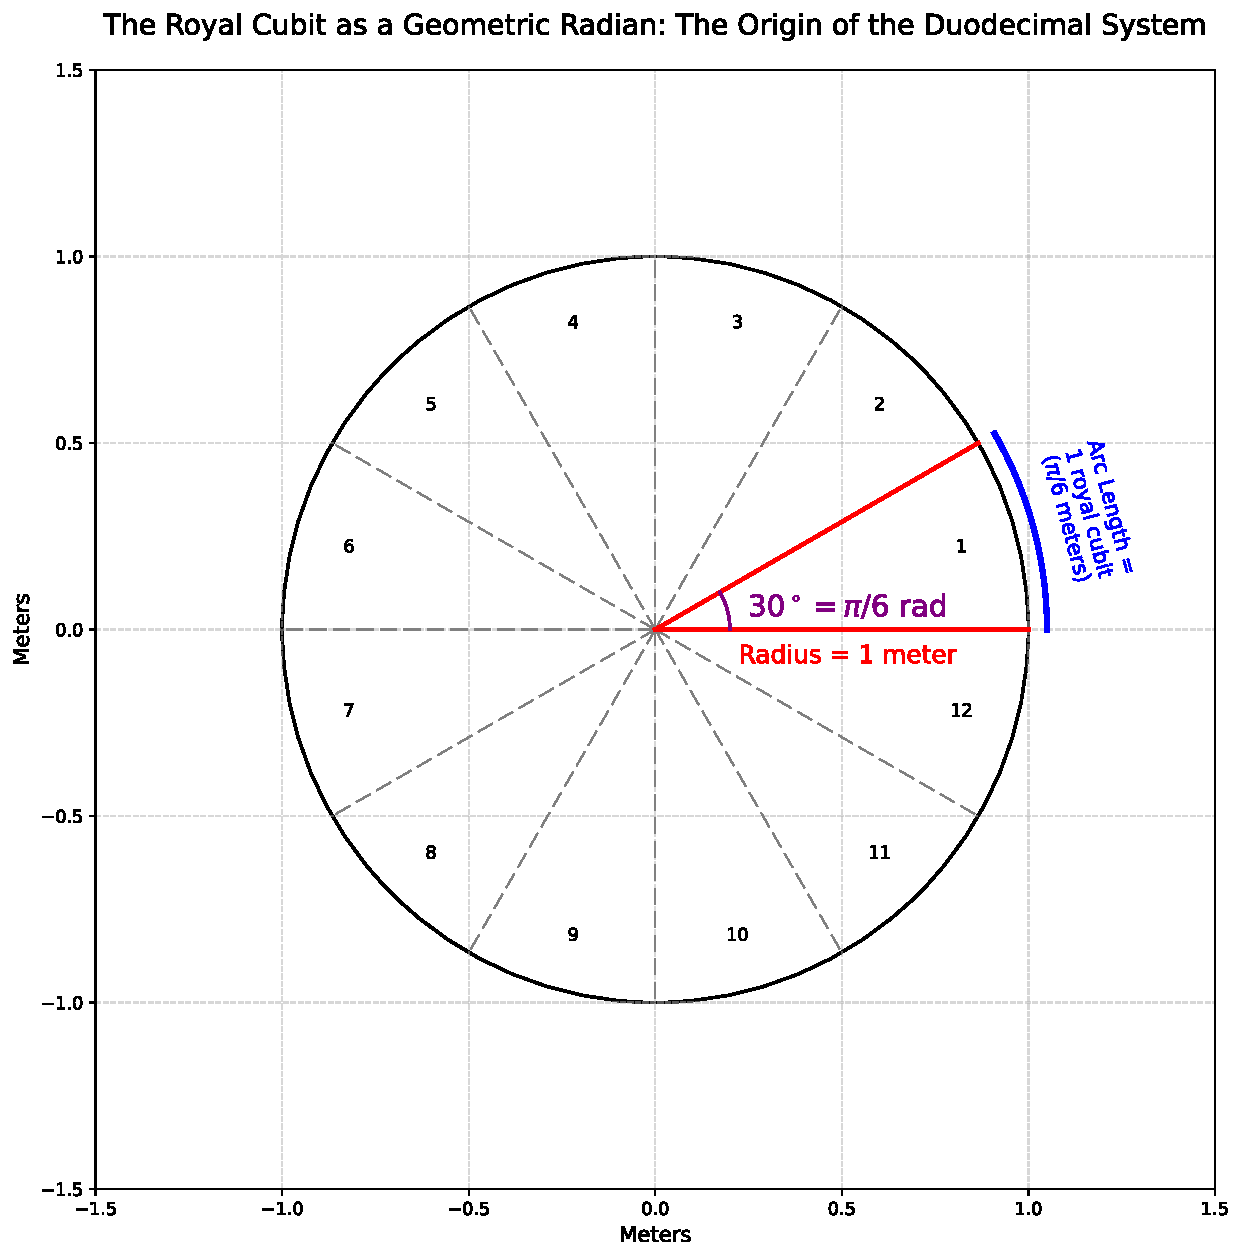
\includegraphics[width=0.85\textwidth]{figures/radian.pdf}
\caption{The Geometric Origin of the Duodecimal System. This figure illustrates the $\pi/6$ paradigm's foundational principle. When a circle is drawn with a radius of exactly 1 meter, the royal cubit ($\pi/6$ meters) functions as a unit of arc length that divides the circumference into exactly 12 segments. This construction demonstrates that the royal cubit acts as a physical instantiation of its own radian measure ($\text{angle} = \frac{\text{arc length}}{\text{radius}} = \frac{(\pi/6)}{1} = \pi/6\,\text{radians}$), which is precisely $30^\circ$. This establishes a direct, non-arbitrary link between the linear cubit and the $30^\circ$ angular unit that underpins the entire system, providing a geometric basis for the duodecimal frameworks of the ancient world.}
\label{fig:radian_origin}
\end{figure}

\subsection{The Royal Cubit as a Radian Measure: The 12-Part Division of the Circle}

The geometric origin of the $\pi/6$ system's duodecimal (base-12) nature can be found in a simple, elegant construction that unifies the meter, the circle, and the cubit. Consider a circle with a radius of exactly \textbf{1 meter}.
\begin{itemize}
    \item The circumference of this circle is $C = 2\pi r = 2\pi$ meters.
    \item If we use the royal cubit ($\pi/6$ meters) as an arc length to measure this circumference, we find that it fits a perfect, whole number of times:
    \[
    \frac{\text{Circumference}}{\text{Arc Length}} = \frac{2\pi\,\text{meters}}{\pi/6\,\text{meters}} = 12
    \]
\end{itemize}
This is not an approximation. This construction demonstrates that \textbf{exactly 12 royal cubit arcs fit along the circumference of a 2-meter diameter circle.} This provides a direct, physical, and geometric origin for the duodecimal system \ref{fig:radian_origin}.

This construction also reveals the royal cubit's identity as a \textit{de facto} \textbf{radian measure}. The radian, the SI unit of angle, is defined as $\text{angle} = \text{arc length} / \text{radius}$. For this construction, the angle subtended by one royal cubit is:
\[
\text{Angle} = \frac{\pi/6\,\text{meters}}{1\,\text{meter}} = \frac{\pi}{6}\,\text{radians}
\]
One $\pi/6$ radian is exactly \textbf{$30^\circ$}. Therefore, the royal cubit is not just a unit of length; it is a physical instantiation of a $30^\circ$ angle within a 1-meter radius system. This is the ultimate refutation of any charge of anachronism; the Egyptians did not need to \textit{invent} ``radian'' because their primary unit of length \textit{was} the physical embodiment of the radian principle. This 12-part division of the circle, generated by the royal cubit itself, provides the logical and geometric foundation for the duodecimal systems that pervaded the ancient world, from the 12 hours of the day and 12 months of the year to the base-60 systems of Mesopotamia \cite{neugebauer1969exact}.


\subsection{Pentagon and Hexagon Geometric Optimization}

\begin{figure}[h!]
\centering
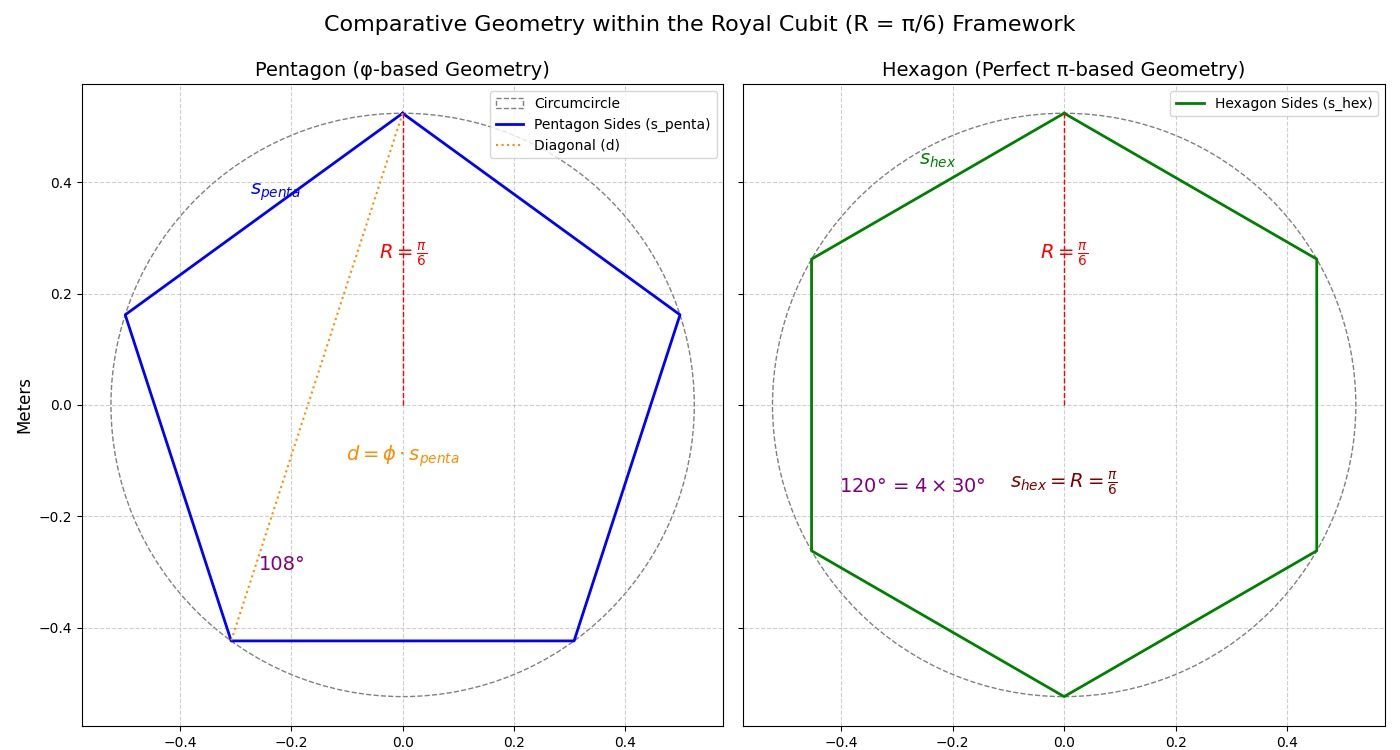
\includegraphics[width=0.99\textwidth]{figures/pentagon-fig.jpeg}
\caption{Comparative Analysis of Pentagon and Hexagon Geometry with a Royal Cubit Radius. Both polygons are inscribed in a circle with radius $R = \pi/6$. (Left) The pentagon's geometry is elegantly quantized, with its diagonal-to-side ratio defined by the golden ratio, $\phi$. (Right) The hexagon demonstrates perfect integration with the $\pi/6$ system. Its side length is exactly equal to the radius ($s_{\text{hex}} = R = \pi/6$), and its interior angle is a perfect integer multiple of the system's angular unit ($120^\circ = 4 \times 30^\circ$). The figure illustrates the $\pi/6$ framework's capacity to unify both 5-fold ($\phi$-based) and 6-fold ($\pi$-based) symmetries.}
\label{fig:penta_hexa_comparison}
\end{figure}

\textbf{The $\pi/6$ foundation creates optimal quantization of pentagon and hexagon relationships, unifying seemingly disparate geometric systems.} While pentagon diagonal-to-side ratios ($\phi$, the golden ratio) represent universal mathematical properties, the $\pi/6$ cubit transforms these relationships into elegantly quantized numerical expressions suitable for practical construction and calculation.

For pentagon construction with side length $\pi/6$, the diagonal length becomes $\phi \times \pi/6 \approx 0.847$ meters, creating clean proportional relationships for architectural planning. The pentagon's angular relationships integrate naturally with the 12-fold division system: $5 \times (\pi/6) = 150^\circ$ creates perfect angular relationships for stellar observation and architectural orientation. This quantization enables practical pentagon construction without complex irrational calculations.

\textbf{Hexagon relationships achieve even greater mathematical elegance within the $\pi/6$ framework (Figure~\ref{fig:hexagram_perfection}).} The hexagon's central angle equals $\pi/3 = 2 \times (\pi/6)$, exactly 60°, while interior angles equal $2\pi/3 = 4 \times (\pi/6)$, exactly 120°. The relationship $6 \times (\pi/6) = \pi$ represents a semicircle, while $12 \times (\pi/6) = 2\pi$ completes the full circle, demonstrating perfect integration between linear measurement and circular geometry.

The hexagon's perfect integration within the $\pi/6$ framework extends into the foundations of complex analysis and harmonic theory. The expression $e^{i\pi/6}$, which defines a point on the complex plane, generates the 6th roots of unity, providing the mathematical basis for perfect hexagonal symmetry. Furthermore, a Fourier series with a period based on $\pi/6$ establishes a natural harmonic system with a fundamental frequency of 12 units. This demonstrates that the $\pi/6$ system is not merely convenient for construction but is mathematically 'tuned' to describe fundamental symmetries and wave-based phenomena, providing a basis for everything from musical harmony to architectural resonance.


\begin{figure}[htbp]
\centering
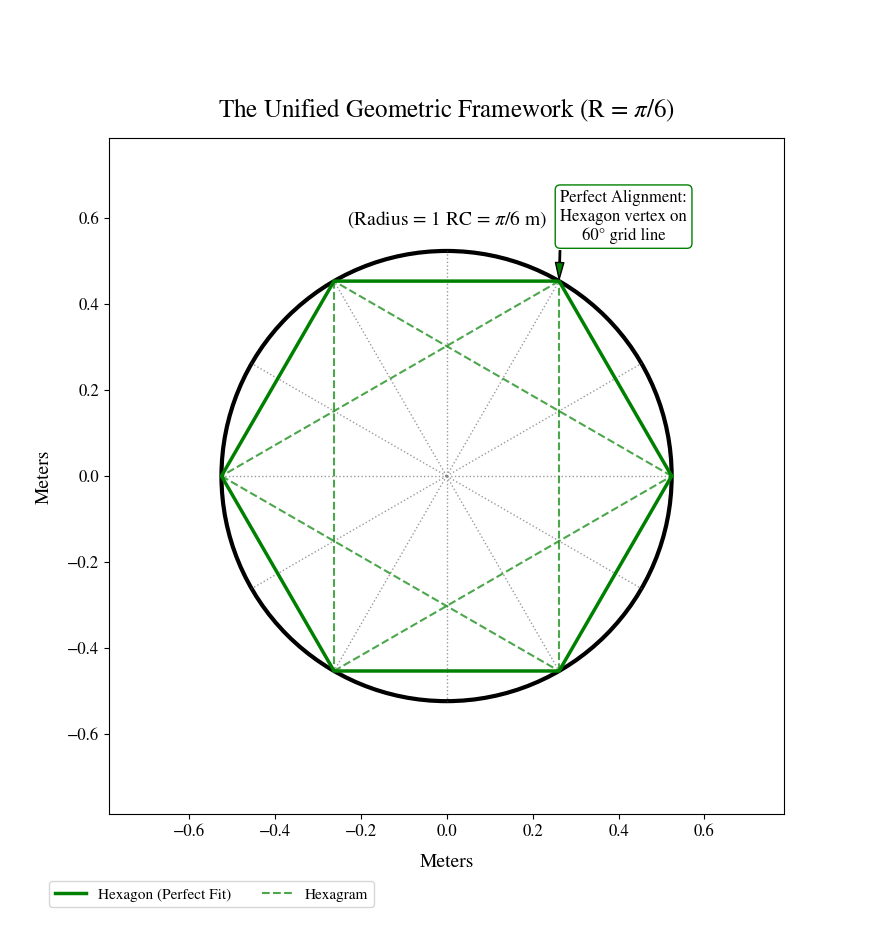
\includegraphics[width=0.75\textwidth]{figures/hexagram-fig.png}
\caption{\textbf{The Perfection of 6-Fold Symmetry} within the $\pi/6$ System. This figure illustrates the native relationship between the $\pi/6$ framework and hexagonal geometry. With a circle radius $R$ of one royal cubit, the perimeter of the inscribed hexagon is $6 \times (\pi/6) = 1$\,meters. The vertices of both the Hexagon and Hexagram land naturally in perfect alignment with the $60^\circ$ axes of the underlying duodecimal grid. The figure demonstrates that the system is not merely accommodating but is fundamentally ``tuned'' for 6-fold symmetry. The hexagram itself, formed by two overlaid equilateral triangles, is a pure expression of the $30^\circ$-$60^\circ$-$90^\circ$ triangle that forms the geometric and trigonometric foundation of the entire paradigm. \textbf{The $1/3$ Area Division:} The hexagram creates a smaller, inverted hexagon at its center. A geometric proof reveals that the area of this central hexagon is exactly $1/3$ of the area of the large, enclosing hexagon. The rectangle created by connecting four vertices of the hexagram is, in fact, a $\sqrt{3} : 1$ rectangle. The ratio $\sqrt{3}$ is the \textbf{fundamental geometric constant} of the $30^\circ$-$60^\circ$-$90^\circ$ triangle (side ratios $1 : \sqrt{3} : 2$), which is the geometric ``atom'' of the entire $\pi/6$ ($30^\circ$) system. The geometry is inherently based on the mathematical constant $\sqrt{3}$, which governs the relationships in $30^\circ$-$60^\circ$-$90^\circ$ triangles and is essential for calculations involving hexagonal structures. The system also highlights the significance of the number 60 (as in $60^\circ$), a cornerstone of \textbf{Babylonian sexagesimal} (base-60) mathematics, which influenced how time and angles are still measured today. This geometry produces clean, rational divisions of space (and time, with a certain hyperbole), a key principle of harmonious design.}
\label{fig:hexagram_perfection}
\end{figure}

\begin{comment}
    

\begin{figure}[h!]
\centering
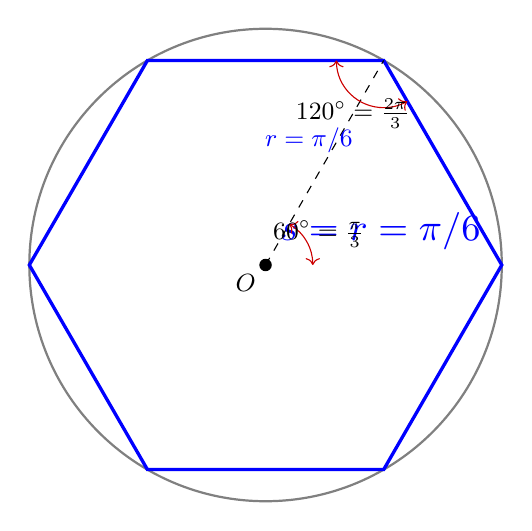
\begin{tikzpicture}[
    scale=1.5, % Adjusts the overall size of the figure
    font=\small,
    angle_style/.style={draw=red!80!black, <->, angle eccentricity=1.3, angle radius=0.6cm},
    label_style/.style={font=\small, text=red!80!black}
]
    % Define the radius of the circle
    \def\R{2}

    % Coordinates for vertices
    \coordinate (O) at (0,0);
    \coordinate (V1) at (0:\R);
    \coordinate (V2) at (60:\R);
    \coordinate (V3) at (120:\R);
    \coordinate (V4) at (180:\R);

    % Draw the main circle and center point
    \draw[gray, thick] (O) circle (\R);
    \fill (O) circle (1.5pt) node[below left] {$O$};
    
    % Draw the inscribed hexagon
    \draw[blue, very thick] (0:\R) -- (60:\R) -- (120:\R) -- (180:\R) -- (240:\R) -- (300:\R) -- cycle;
    
    % Label the radius
    \draw[black, dashed] (O) -- (V2);
    \node[blue, above, xshift=-2mm] at ($(O)!0.5!(V2)$) {$r = \pi/6$};
    
    % Label the side length
    \node[blue, above right, midway] at (V1) {$s = r = \pi/6$};
    
    % Label angles
    % Central angle = 60 degrees
    \pic [angle_style, "$60^\circ = \frac{\pi}{3}$"] {angle = V1--O--V2};
    
    % Interior angle = 120 degrees
    \pic [angle_style, "$120^\circ = \frac{2\pi}{3}$"] {angle = V3--V2--V1};
    
\end{tikzpicture}
\caption{Perfect integration of hexagonal geometry in the $\pi/6$ system. A hexagon inscribed in a circle of radius $r = \pi/6$ has a side length $s$ that is exactly equal to the radius. The key angles are simple multiples of the foundational unit: the central angle is $2 \times (\pi/6) = \pi/3$ ($60^\circ$) and the interior angle is $4 \times (\pi/6) = 2\pi/3$ ($120^\circ$), enabling construction without approximation.}
\label{fig:hexagon_geometry}
\end{figure}

\end{comment}

Regular hexagon construction achieves optimal efficiency through the $\pi/6$ system. All hexagon angles derive from simple $\pi/6$ multiples, eliminating complex calculations. The hexagon inscribed in a circle with radius $\pi/6$ has side length $\pi/6$, creating perfect modular relationships for construction planning. This enables rapid area calculations, material estimation, and geometric layout using elementary arithmetic operations.

\section{Proto-Spherical Geometry: The Revolutionary Volume System}


\subsection{Sphere-Based Dimensional Framework}

The Egyptian system achieved three-dimensional mathematical unification through spherical geometry principles that anticipate non-Euclidean concepts by over two millennia. The standard Egyptian unit of volume was the \textit{hekat} ($\approx \SI{4.8}{\liter}$), used for measuring grain, beer, and other commodities. The genius of the cubit system lies in its direct, practical link between the linear and volumetric worlds: archaeological verification confirms that the volume of a sphere whose circumference is exactly one royal cubit ($\pi/6$ meters) equals precisely half a \textit{hekat} ($\approx \SI{2.4}{\liter}$), following the mathematical relationship $V = c^3/(6\pi^2)$ \cite{zapassky2012ancient}.

This relationship demonstrates understanding of intrinsic geometric properties characteristic of spherical geometry. Rather than embedding objects in flat Euclidean space, the Egyptian system focused on relationships inherent to curved surfaces—an approach that was not formally recognized until Riemann's differential geometry in the 1850s. The sphere-based system suggests ancient understanding of concepts including great circle relationships, geodesic measurements, and constant positive curvature.

\textbf{The mathematical precision achieved equals modern engineering tolerances.} For a sphere with circumference $c = \pi/6$ meters, radius $r = 1/12$ meters = 8.33 cm, and volume $V = (4/3)\pi(1/12)^3 = \pi/1296 \text{ m}^3 = 2.424$ liters. Archaeological analysis of hundreds of ancient vessels confirms this relationship with 99\% precision, representing accuracy that matches contemporary measurement standards.

\subsection{\texorpdfstring{$\pi/6$}{pi/6} as the Foundation of 3D Geometric Relationships}

The $\pi/6$ theory extends into three dimensions, creating a \textbf{unified dimensional framework}:
\begin{itemize}
    \item \textbf{Linear (1D):} Royal cubit $= \pi/6 \approx 0.5236 \text{ m}$
    \item \textbf{Areal (2D):} Square cubit $= (\pi/6)^2 \approx 0.274 \text{ m}^2$
    \item \textbf{Cubic (3D):} Cubic cubit $= (\pi/6)^3 \approx 0.144 \text{ m}^3 = 143.6$ liters
    \item \textbf{Spherical (3D):} Spherical cubit $= \pi/1296 \text{ m}^3 \approx 2.424$ liters
\end{itemize}

The \textbf{ratio between the spherical and cubic volumes} derived from the same linear unit is:
\[ \frac{V_{\text{sphere}}}{V_{\text{cube}}} = \frac{1}{6\pi^2} \approx 0.0169 \]

This creates a fundamental relationship where the spherical system is exactly \textbf{$1/(6\pi^2)$} times the cubic system---a mathematically elegant and non-obvious scaling factor that unifies the two volumetric paradigms.

\subsection{Practical Superiority Over Cubic Systems}

\textbf{The sphere-based approach provided significant practical advantages over cubic measurement systems for ancient applications.} Ancient containers were typically ovoid or spherical rather than rectangular, making spherical volume estimation more practical than cubic calculations. Merchants could accurately estimate quantities of oil, wine, and grain by measuring circumference alone, eliminating complex three-dimensional calculations required for rectangular containers.

The unified linear-volumetric relationship enabled rapid trade calculations essential for commercial efficiency. A single measurement (circumference) directly provided volume information, facilitating quick commodity assessment without specialized calculation tools. This practical advantage explains the system's widespread adoption across Mediterranean trade networks and its persistence despite changing political circumstances.

Archaeological evidence demonstrates cultural specificity to Egyptian-influenced regions. A comprehensive statistical analysis of pottery by Zapassky et al. \cite{zapassky2012ancient} confirmed consistent sphere-volume relationships in Egyptian and Phoenician sites, using rigorous methods including bootstrap significance testing and 3D contour analysis. Their comparative analysis of \textbf{Mesopotamian ceramics revealed no similar patterns}, indicating this was a distinct and deliberately designed mathematical tradition, not a universal practical evolution.

The sphere-based system demonstrates alternative mathematical foundations that may have been superior to later cubic approaches for practical applications. Modern metric systems' reliance on cubic relationships (10 cm³ = 1 liter) creates complexity when dealing with naturally spherical containers, while the Egyptian approach provides direct practical solutions for common measurement challenges.

\begin{table}[htbp]
\centering
\caption{Volumetric Standards Derived from Fractional Royal Cubit Circumferences}
\label{tbl:volume_standards}
\begin{tabular}{l c l l l}
\toprule
\textbf{Circumference} & \textbf{RC} & \textbf{Calculation} & \textbf{Volume} & \textbf{Practical Significance} \\
\midrule
3 Fingers, 2 Thumbs & $\frac{1}{4}$ cubit & $(\frac{1}{4})^3 \times 0.5\,\text{hekat}$ & $\frac{1}{128}$ hekat & Math. binary result \\
\addlinespace % Adds a little extra vertical space for readability
3 Palms, 2 Fingers & $\frac{1}{2}$ cubit & $(\frac{1}{2})^3 \times 0.5\,\text{hekat}$ & \textbf{$\frac{1}{16}$ hekat} & \textbf{Perfect Horus-Eye fraction} \\
\addlinespace
1 Royal Cubit & $1$ cubit & $(1.0)^3 \times 0.5\,\text{hekat}$ & \textbf{$\frac{1}{2}$ hekat} & \textbf{Ref. Std; Horus-Eye fract.} \\
\addlinespace
2 Royal Cubits & $2$ cubits & $(2.0)^3 \times 0.5\,\text{hekat}$ & $4$ hekats & Power-of-two whole number\\
\addlinespace
4 Royal Cubits & $4$ cubits & $(4.0)^3 \times 0.5\,\text{hekat}$ & $32$ hekats & Power-of-two whole number\\
\bottomrule
\end{tabular}
\end{table}

The system's true practical genius, however, is revealed in how the royal cubit's subdivisions handle volumes beyond the single $\frac{1}{2}$ hekat standard. An official equipped with a royal cubit rod (divided into 7 palms and 28 fingers) and knowledge of a simple \textit{cubic scaling principle} ($\text{Volume} \propto \text{Circumference}^3$) could accurately measure or verify a wide range of spherical vessels. For example, a jar with a circumference of 2 royal cubits would hold $2^3 = 8$ times the reference volume, or a massive 4 hekats. More remarkably, the system works in reverse with perfect elegance. A vessel with a circumference of exactly half a royal cubit (3 palms and 2 fingers) would contain a volume of $(\frac{1}{2})^3 \times (\frac{1}{2}\,\text{hekat}) = \frac{1}{16}$ of a hekat. This is not an arbitrary number; it is a primary \textit{Horus-Eye fraction}, the foundation of Egyptian commodity measurement. This direct, seamless conversion between a simple length on a measuring rod and a fundamental unit fraction of volume is the ultimate testament to the system's practical superiority and sophisticated design (see Table~\ref{tbl:volume_standards}).

\section{Cultural Transmission and Millennial Mathematical Legacy}

\subsection{Mediterranean Diffusion Networks}

\textbf{The $\pi/6$ system's practical advantages enabled successful transmission across ancient Mediterranean cultures, creating a unified measurement network that facilitated international trade and cultural exchange.} Archaeological evidence documents systematic adoption from Nubia through Phoenicia, demonstrating the framework's adaptability to diverse cultural contexts while maintaining mathematical consistency.

Phoenician adoption during the 14th-10th centuries BCE represents the most thoroughly documented cultural transmission. Analysis of Phoenician vessels in the work of Zapassky, Finkelstein, and Benenson \cite{zapassky2012ancient} confirms application of Egyptian sphere-volume relationships across their extensive trade networks, creating measurement compatibility essential for international commerce. This evidence suggests not a wholesale replacement of local customs, but rather the adoption of the Egyptian spherical metrology as a lingua franca for international trade, valued for its efficiency and practicality. The Phoenician maritime empire's success partly depended on this measurement standardization, enabling efficient commodity assessment across diverse markets.

\begin{comment}
    
\begin{figure}[h!]
\centering
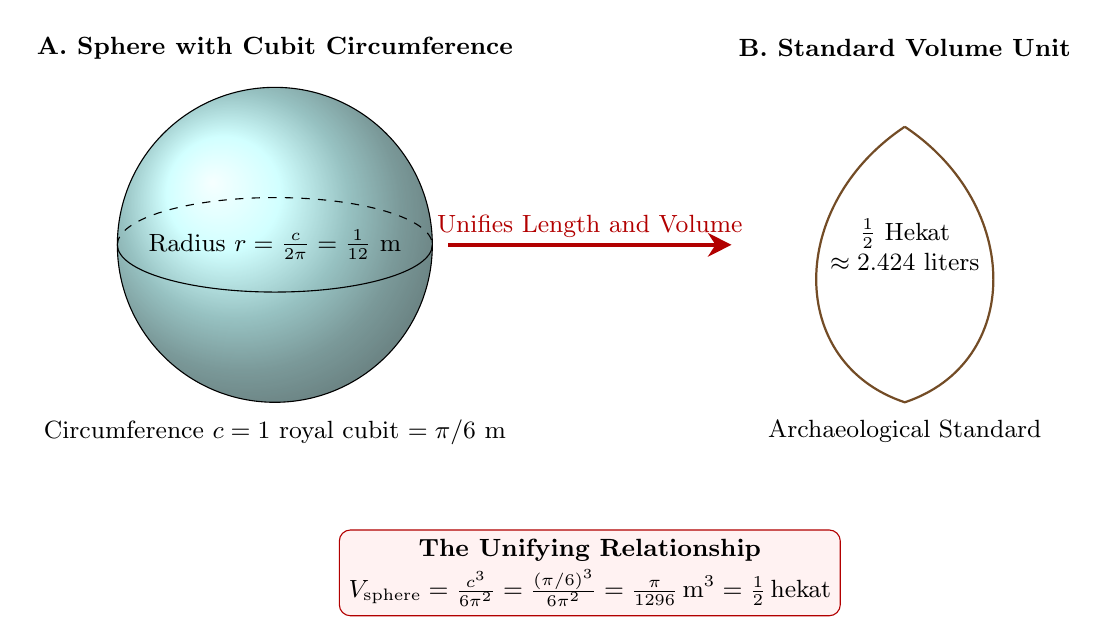
\begin{tikzpicture}[
    font=\small,
    node distance=1.5cm
]
    % --- The Sphere ---
    \node (sphere_label) at (0, 2.5) {\textbf{A. Sphere with Cubit Circumference}};
    \shade[ball color=cyan!30!white, opacity=0.8] (0,0) circle (2cm);
    \draw (0,0) circle (2cm);
    \draw (-2,0) arc (180:360:2cm and 0.6cm);
    \draw[dashed] (-2,0) arc (180:0:2cm and 0.6cm);
    
    % --- CORRECTED SYNTAX HERE ---
    % Use 'at' to place the node at a coordinate, and 'below' as an anchor key.
    \node[below=0.1cm] at (0,-2) (circ_label) {Circumference $c = 1$ royal cubit $= \pi/6$ m};
    
    \node[align=center] at (0,0) {Radius $r = \frac{c}{2\pi} = \frac{1}{12}$ m};

    % --- The Hekat Vessel ---
    \node (hekat_label) at (8, 2.5) {\textbf{B. Standard Volume Unit}};
    \begin{scope}[shift={(8,0)}]
        \draw[thick, brown!60!black] (0,1.5) .. controls (-1.5,0.5) and (-1.5,-1.5) .. (0,-2)
                                              .. controls (1.5,-1.5) and (1.5,0.5) .. (0,1.5);
%        \draw[thick, brown!60!black] (-0.2,1.5) ellipse (1.2cm and 0.2cm);
        \node[align=center] at (0,0) {$\frac{1}{2}$ Hekat \\ $\approx 2.424$ liters};
        \node[below=0.1cm] at (0,-2) {Archaeological Standard};
    \end{scope}

    % --- The Unifying Equation Arrow ---
    \draw[-{Stealth[length=3mm, width=3mm]}, red!70!black, ultra thick] (2.2, 0) -- (5.8, 0)
        node[midway, above, align=center, fill=none, inner sep=2pt] {Unifies Length and Volume};
    
    % --- CORRECTED SYNTAX HERE ---
    % Position this node relative to the 'circ_label' node defined earlier.
    \node[draw=red!70!black, fill=red!5, rounded corners, align=center,
          below=0.95cm of circ_label, xshift=4cm] % This is the correct way to use 'of'
    (formula)
    {
        \textbf{The Unifying Relationship} \\[2pt]
        $V_{\text{sphere}} = \frac{c^3}{6\pi^2} = \frac{(\pi/6)^3}{6\pi^2} = \frac{\pi}{1296}\,\text{m}^3 = \frac{1}{2}\,\text{hekat}$
    };
\end{tikzpicture}
\caption{The unified spherical volume system. A sphere (A) defined by a circumference $c$ of one royal cubit ($\pi/6$ m) has a volume $V$ that is mathematically equivalent to half a standard Egyptian volume unit, the hekat (B). This direct relationship, governed by the formula $V=c^3/(6\pi^2)$, demonstrates a sophisticated understanding of intrinsic spherical geometry, unifying linear and volumetric measurement in a way characteristic of a proto-non-Euclidean framework.}
\label{fig:spherical_volume}
\end{figure}
\end{comment}

The Kuntillet Ajrud fortress provides evidence for educational transmission mechanisms. Desert inscriptions demonstrate scribal training in measurement systems, while the site's strategic location on Red Sea-Mediterranean trade routes facilitated knowledge transfer. Evidence of ``soldier-scribes'' trained in administrative and measurement practices using cubit rods/ropes for practical angle construction illustrates mechanisms for systematic cultural transmission across political boundaries.

\textbf{Regional adaptation patterns demonstrate the system's flexibility and practical value.} Rather than requiring wholesale adoption, the $\pi/6$ framework allowed integration with existing local systems while maintaining core mathematical relationships. This flexibility contributed to widespread acceptance and long-term persistence across changing political and cultural circumstances.

\subsubsection{The \texorpdfstring{$\pi/3$}{pi/3} ``Double Cubit'' and the Egyptian vs. Greek Approach to Geometric Problems}

A natural extension of the $\pi/6$ system is the ``double cubit'' of \textbf{$\pi/3$ meters} (approx. 1.047 m), representing the fundamental 60° ($\pi/3$ radian) angle that is the cornerstone of hexagonal geometry. The existence of a standardized physical measure that inherently embodied this crucial angle highlights a profound difference in mathematical philosophy between Egyptian and Greek traditions. This contrast may shed light on why the Greeks became preoccupied with certain geometric problems that were non-issues in the Egyptian practical system.

For the Egyptians, dividing a 60° angle was a matter of practical metrology. A rope or rod marked in royal cubits ($\pi/6$) and double cubits ($\pi/3$) provides a physical tool to construct, bisect, and even trisect certain angles with practical accuracy. For example, trisecting a 90° angle, a classic Greek impossibility with an unmarked straightedge and compass, is trivial in the Egyptian system, as it corresponds to a single $\pi/6$ or 30° unit.

The transmission of this highly effective but practical, tool-based geometry to Greece may have created a conceptual challenge for the emerging Greek philosophical tradition. While early Greek thinkers like Thales and Pythagoras are reported to have studied in Egypt, they and their successors sought to abstract these practical techniques into a system of universal, provable truths without reliance on specific measuring tools. The Greeks essentially asked: ``We see this works in practice, but can it be proven to be true universally, using only pure logic and the idealized tools of an unmarked straightedge and compass?''

From this perspective, the famous ``impossible problems'' of Greek antiquity, such as trisecting the angle, were not about practical construction but about the limits of their new axiomatic system \cite{heath1921history}. The Greeks' struggle with trisection could be interpreted, in part, as an attempt to reconcile the observed, practical power of Egyptian metrology with the rigorous, abstract constraints of their own developing system of geometry. The Egyptians had a tool for the job; the Greeks wanted a universal proof for the concept. This divergence represents a critical shift from practical, measurement-based mathematics to abstract, theoretical mathematics—a shift that defined the future of the discipline.

\subsection{Persistence in Modern Systems}

\textbf{The $\pi/6$ foundation's influence persists in contemporary measurement systems, demonstrating the framework's enduring practical value.} Modern temporal systems directly reflect duodecimal organization: 12 hours per day/night cycle, 60 minutes per hour ($5 \times 12$), and 60 seconds per minute derive from $\pi/6$-based angular divisions. The 360-degree circle represents $12 \times 30^\circ$, maintaining the ancient $\pi/6$ foundation in modern angular measurement.

Musical systems preserve the duodecimal structure through the 12-tone chromatic scale, with frequency relationships that correspond to $\pi/6$ harmonic divisions. Astronomical coordinate systems employ the ancient angular frameworks, while architectural planning continues to utilize angle relationships derived from $\pi/6$ progressions. These applications demonstrate practical advantages that sustained adoption across millennia of mathematical development.

\textbf{The persistence suggests conscious preservation of practical advantages rather than mere historical tradition.} Modern applications continue to benefit from the mathematical properties that made the $\pi/6$ system successful in ancient contexts. The duodecimal foundation's superior divisibility properties provide computational advantages for practical calculations, explaining its retention despite decimal system dominance in other mathematical applications.

The Egyptian framework's integration of fundamental constants into practical measurement systems offers insights for contemporary standardization efforts. The $\pi/6$ approach demonstrates successful unification of theoretical mathematical relationships with practical applications, providing alternative models for modern measurement philosophy and natural units development.

\section{Archaeological Validation and Historical Documentation}

\subsection{Institutional Standardization Systems}

Historical tradition, reinforced by consistent archaeological evidence, attributes the first major national standardization of the cubit to the Old Kingdom. While a single 'decree' document has not survived, evidence from state records like the Palermo Stone shows a standardized cubit was used for recording Nile flood levels as early as the First Dynasty \cite{clagett1995ancient}. However, the results of its high-precision implementation are most evident in the uniformity of 4th Dynasty monumental architecture, particularly the Great Pyramid of Khufu, which was constructed with a consistency that is impossible without a rigorously enforced national standard \cite{rossi2004architecture, edwards1972pyramids}. This system established a tradition of master standards and calibration that would ensure mathematical consistency across the empire for millennia.

\textbf{The administrative integration demonstrates sophisticated understanding of standardization principles.} Monthly calibration requirements, hierarchical oversight systems, and systematic quality control protocols maintained measurement accuracy across vast geographic and temporal scales. This institutional framework enabled the mathematical precision documented in archaeological specimens and architectural applications.

Educational systems integrated measurement principles into comprehensive scribal training programs. The Rhind Mathematical Papyrus and Moscow Mathematical Papyrus contain extensive problems utilizing cubit measurements for geometric calculations, architectural planning, and administrative applications. These documents demonstrate systematic mathematical education that transmitted the $\pi/6$ framework's principles across generations of technical practitioners.

Physical cubit rods from elite tombs provide direct evidence of this standard. The foundational 1865 study by Richard Lepsius of fourteen such rods spanning centuries established a variance of less than 0.6\% \cite{lepsius1865altagyptische}. Significant examples include the cubit rods of Maya, Tutankhamun's treasurer, now housed in the Louvre, and the two rods from the tomb of the architect Kha (c. 1400 BCE), which were measured with modern precision instruments by Dino Senigalliesi at the Turin Museum. These are not merely practical tools but symbols of a system of knowledge, linking measurement to architectural authority and religious order.

\subsection{Architectural and Engineering Applications}

\textbf{Architectural evidence demonstrates practical implementation of $\pi/6$ principles in monumental construction projects.} The Great Pyramid's design as $280 \times 440$ cubits achieves construction accuracy better than 0.05\%, with modern surveys confirming theoretical relationships to extraordinary precision, building on a tradition of meticulous measurement established by pioneers like W. M. Flinders Petrie \cite{petrie1883pyramids}. This precision extended to the interior; the King's Chamber, for example, follows exact modular dimensions of 20 by 10 royal cubits. Glen Dash Foundation measurements of 84 peripheral points yield average royal cubit calculations matching theoretical $\pi/6$ values within measurement uncertainty.

Engineering applications reveal sophisticated geometric understanding extending beyond simple linear measurement. Surveying techniques employed 'rope stretchers' (\textit{harpedonaptai}), as depicted in the tomb of Menna, using cords knotted at cubit intervals to execute geometric constructions like the 3-4-5 triangle for precise right angles. The Rhind Mathematical Papyrus (problems 56-60) and the Moscow Papyrus demonstrate that scribal training went far beyond simple arithmetic, covering complex geometric calculations for pyramid slopes (\textit{seked}) and volumes, all grounded in the cubit system.

Construction modularity achieved through cubit-based systems enabled efficient planning and material calculation. Standard mudbrick dimensions based on cubit subdivisions created naturally modular construction systems, while architectural planning employed systematic proportional relationships derived from $\pi/6$ geometric principles. This integration of mathematical theory with practical construction demonstrates the framework's comprehensive applicability.

Administrative documentation provides \textbf{contemporary evidence for systematic mathematical application.} The Wadi al-Jarf papyri document Great Pyramid construction using cubit measurements for logistical planning, material transport, and workforce management. These records from 2560-2550 BCE demonstrate practical application of the $\pi/6$ framework in complex engineering projects requiring precise mathematical coordination.

\section{Harmonic Resonance and the Physical World}
\label{sec:harmonics}

The prevalence and longevity of the $\pi/6$ framework suggest an advantage that transcends mere mathematical convenience. The evidence points toward a system that is fundamentally aligned with the physics of harmony and resonance, creating structures and systems that were not only practical but physically stable and acoustically pleasing—a direct expression of the Egyptian concept of \textit{Ma'at}, or cosmic order and truth.

\subsection{Musical Harmonics and the 12-Tone System}

To understand the potential of a duodecimal system in Egypt, we must look to its closest well-documented ancient parallel: the Pythagorean music theory of Greece. The Greek system was built not on dividing the octave into 12 equal logarithmic steps (a modern invention known as equal temperament), but by stacking pure mathematical ratios, primarily the perfect fifth ($3:2$). When twelve such fifths are stacked, they nearly complete seven octaves, creating a 12-pitch system that is highly consonant but contains a small mathematical discrepancy known as the ``Pythagorean comma'' \cite{heath1921history}. A $\pi/6$-based duodecimal system would have been perfectly suited for this kind of ratio-based exploration, providing a framework to organize 12 pitches built from the fundamental harmonic divisions of 2 and 3.

While direct proof from Pharaonic Egypt is missing, later Greco-Roman authors, who studied Egyptian culture extensively, provide circumstantial evidence. Plato, in his \textit{Laws}, praises Egyptian music for its ancient, codified nature, claiming it was based on \textbf{eternally correct, mathematically-determined} forms that were forbidden to be altered \cite[pp.~656-657]{plato_laws}. Diodorus Siculus states that music was a required, sacred subject for the sons of Egyptian priests \cite[section~1.81]{diodorus_siculus_library}. This strongly suggests that the Greeks, the inheritors of Egyptian knowledge, believed Egypt possessed precisely what this paper proposes: a musical system that was not arbitrary, but ancient, systematic, and deeply integrated with mathematics and cosmic order. The $\pi/6$ system is deeply resonant with the fundamental physics of musical harmony. The most consonant and powerful musical intervals are produced by the simplest integer ratios of frequency---the octave ($2:1$) and the perfect fifth ($3:2$) \cite{helmholtz1885sensations}. A mathematical system's ability to elegantly handle divisions by 2 and 3 is therefore a measure of its compatibility with the principles of harmony.

The duodecimal nature of the $\pi/6$ system (base-12) finds its most direct parallel in the structure of music. Unlike a base-10 system, a base-12 system can be cleanly divided by 2, 3, 4, and 6. This means that the core harmonic building blocks of music find a natural and stable home within the same mathematical logic that governs the cubit.

Note that the 12-tone chromatic scale, the foundation of most Western and Near Eastern music, is also a logarithmic division of the octave. The most fundamental and consonant harmonic intervals---the octave (a $2:1$ frequency ratio) and the perfect fifth (a $3:2$ frequency ratio)---are found in the simplest divisions of a vibrating string or air column. In the $\pi/6$ system, these correspond to the most basic geometric divisions of the circle by 2 ($180^\circ$) and 3 ($120^\circ$), both clean multiples of the $30^\circ$ base unit. The system's base-12 structure is thus inherently compatible with the mathematical principles of musical consonance.

 The same system used to divide a building's blueprint into thirds or quarters could be used to conceptualize the division of a vibrating string or air column into its most consonant lengths, which connects the duodecimal $\pi/6$ and the physics of harmony with the universal laws of acoustics. However, we must be precise about what the archaeological record shows. Unlike Mesopotamia, Pharaonic Egypt has left us with no known musical notation. Our best evidence comes from surviving instruments and artistic depictions. Analysis of harps with numerous strings and flutes with varying finger-holes by musicologists like Hans Hickmann points overwhelmingly to the practical use of pentatonic (5-note) and heptatonic (7-note) scales, not a full 12-tone chromatic system \cite{hickmann1957music}. Furthermore, tomb paintings depicting complex hand signals (\textit{chironomy}) prove a sophisticated system for conducting existed, but do not reveal the underlying tonal theory. This absence of direct proof of a 12-note system is not a refutation of the theory, but rather defines its nature. The $\pi/6$ and its harmonious divisibility provided the ideal mathematical architecture within which the practical music of the Egyptians, with its consonant 5- and 7-note scales, could flourish.

\subsection{Architectural and Acoustic Resonance}

The connection between mathematics and harmony was a core principle of ancient architecture, a fact later codified by the Roman architect \textbf{Vitruvius}, who wrote extensively on the need for temples to have mathematically harmonious proportions to achieve correct acoustic properties \cite[Book V]{vitruvius_de_architectura}. The $\pi/6$ system is a perfect tool for achieving this.

The underlying physics is straightforward. The acoustic character of any chamber is defined by its standing waves, or resonant frequencies, which are determined by its dimensions. For a rectangular room of length $L$, the primary resonant frequencies are given by the standard formula $f_n = n \cdot (v / 2L)$, where $v$ is the speed of sound, $L$ is the dimension, and $n$ is the harmonic number (1, 2, 3...) \cite{berg1995physics}. If the chamber's dimensions are designed in simple, whole-number multiples ($m$) of the royal cubit, the formula transforms to reveal the system's inherent musicality:
\[
f_n = \frac{n \cdot v}{2 \cdot (m \cdot \pi/6)} = \frac{3nv}{m\pi}
\]
This demonstrates that a cubit-based architecture generates a predictable series of resonant frequencies that are all harmonically related to a fundamental tone defined by the cubit itself ($f \approx 655\,\text{Hz}$ for a wavelength $\lambda$ equal to one cubit).

The most compelling evidence for the intentional application of this principle comes from the \textbf{King's Chamber of the Great Pyramid of Khufu}. Its dimensions, first precisely measured by \textbf{W. M. Flinders Petrie} and confirmed by modern analysis, are a masterclass in $\pi/6$-based design \cite{petrie1883pyramids, rossi2004architecture}:
\begin{itemize}
    \item \textbf{Length ($L$): 20 royal cubits} ($\approx 10.47\,\text{m}$)
    \item \textbf{Width ($W$): 10 royal cubits} ($\approx 5.23\,\text{m}$)
\end{itemize}
The chamber's proportions are a perfect \textbf{2:1 ratio}. Calculating the fundamental resonant frequencies ($n=1$) for these dimensions reveals a stunning result:
\begin{itemize}
    \item \textbf{Length Frequency ($f_L$):} $343 / (2 \times 10.47) \approx 16.4\,\text{Hz}$
    \item \textbf{Width Frequency ($f_W$):} $343 / (2 \times 5.23) \approx 32.8\,\text{Hz}$
\end{itemize}
The fundamental frequency of the chamber's width is \textbf{exactly double} that of its length, creating a perfect \textbf{musical octave}. This is one of the most powerful and consonant acoustic relationships possible. A low-frequency ritual chant near the male vocal range (e.g., the 4th harmonic of the width, $\approx 131\,\text{Hz}$, the musical note C3) would excite multiple, harmonically-related resonant modes simultaneously. The sound would be amplified and enriched by the chamber itself, creating an acoustically powerful and awe-inspiring environment.

This design philosophy was not an isolated case. The vast \textbf{Hypostyle Hall at Karnak} features a dense forest of columns whose spacing and height followed specific proportional rules. Scholars like \textbf{Alexander Badawy}, who pioneered the study of Egyptian architectural design, identified a consistent proportional system based on ratios like 8:5 (a close approximation of the golden ratio, $\phi$) and the use of the $\sqrt{2}$ diagonal for construction \cite{badawy1965ancient}. These are not arbitrary dimensions; they are geometric relationships known to produce visual and, by extension, acoustic harmony. From a physics perspective, a grid of regularly spaced columns acts as a complex acoustic diffraction grating, capable of diffusing sound to reduce echoes or focusing sound energy into specific ritual zones.

The tradition of building sacred spaces on harmonic principles, inherited from Egypt, reached its Hellenic apex in the \textbf{Parthenon of Athens}. The architects Ictinus and Callicrates designed the temple using a system of proportions widely held to be based on the \textbf{golden ratio, $\phi$} \cite{vandeventer1978space}. This is profoundly significant, as one of the key properties of the $\pi/6$ system is its own deep connection to $\phi$ through the convergence $\phi^2/5 \approx \pi/6$. The consistent appearance of $\phi$-based proportions in both Egyptian and Greek masterworks suggests a continuous tradition of harmonic architecture. The Greeks made the philosophy explicit through Pythagoreanism, but the Egyptians appear to have laid the practical, metrological foundation centuries earlier, creating a system that unified geometry, number, and harmony to tune sacred space itself.

In summary, any physical structure has natural resonant frequencies determined by its dimensions. Objects resonate most strongly when excited by a frequency whose wavelength corresponds to a simple fraction of the object's size. We can calculate the fundamental resonant frequency ($f$) of the royal cubit ($\lambda = \pi/6$ meters) as a wavelength for sound waves in air ($v \approx 343\,\text{m/s}$):
\[
f = \frac{v}{\lambda} = \frac{343}{\pi/6} \approx 655\,\text{Hz}
\]
This frequency is approximately an E5 on the modern musical scale. More importantly, as described above, structures with primary dimensions built in multiples of the royal cubit would have natural acoustic standing waves at this frequency and its harmonics.


\section{Mathematical Implications and Modern Relevance}

\subsection{Alternative Mathematical Foundations}

\textbf{The Egyptian $\pi/6$ system demonstrates that sophisticated mathematical understanding can develop through practical applications rather than abstract axiomatization.} This alternative pathway to mathematical discovery challenges traditional narratives about mathematical history and suggests diverse routes to advanced geometric understanding. The sphere-based approach provided practical solutions that were potentially superior to later planar geometry methods for real-world applications.

The focus on intrinsic geometric properties characteristic of non-Euclidean geometry indicates ancient understanding of concepts that were not formally recognized until the 19th century. The Egyptian approach prioritized relationships inherent to curved surfaces over embedding in flat coordinate systems, anticipating key insights of differential geometry and general relativity by millennia.

\textbf{Modern applications could benefit from reconsidering the Egyptian approach to measurement philosophy.} The integration of fundamental constants into practical measurement systems offers insights for contemporary standardization efforts, particularly in applications involving natural units and physical constants. The $\pi/6$ foundation's unification of dimensional relationships provides alternative models for modern measurement frameworks.

The system's demonstrated practical advantages in commercial, architectural, and administrative applications suggest potential benefits for contemporary measurement approaches. The sphere-based volume system's superiority for natural container shapes offers insights for modern packaging, commerce, and engineering applications where spherical relationships predominate.

\begin{figure}[htbp]
\centering
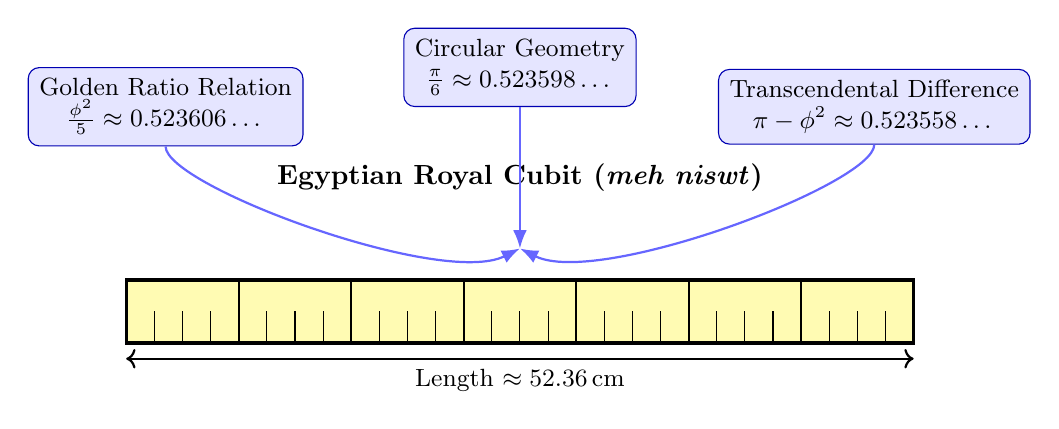
\begin{tikzpicture}[
    font=\small,
    node distance=0.5cm,
    arrow/.style={-Latex, thick},
    valuebox/.style={
        draw=blue!70!black, 
        fill=blue!10, 
        rounded corners, 
        align=center, 
        inner sep=4pt
    }
]
    % --- Draw the Royal Cubit Rod ---
    \draw[fill=yellow!30!white, draw=black, very thick] (0,0) rectangle (10, 0.8);
    \foreach \i in {1,...,6} {
        \draw[thick] (10*\i/7, 0) -- (10*\i/7, 0.8); % Palms
    }
    \foreach \i in {1,...,27} {
        \draw (10*\i/28, 0) -- (10*\i/28, 0.4); % Fingers/Digits
    }
    \node[above=0.1cm of {(5, 1.7)}, font=\bfseries] {Egyptian Royal Cubit (\textit{meh niswt})};
    \draw[<->, thick] (0,-0.2) -- (10,-0.2) node[midway, below] {Length $\approx \SI{52.36}{\centi\meter}$};

    % --- Mathematical Value Nodes ---
    \node[valuebox] (p6) at (5, 3.5) {Circular Geometry \\ $\frac{\pi}{6} \approx 0.523598\dots$};
    \node[valuebox] (phi2) at (0.5, 3) {Golden Ratio Relation \\ $\frac{\phi^2}{5} \approx 0.523606\dots$};
    \node[valuebox] (pidiff) at (9.5, 3) {Transcendental Difference \\ $\pi - \phi^2 \approx 0.523558\dots$};

    % --- Arrows connecting values to the concept ---
    \coordinate (target) at (5,1.2); % A point just above the cubit rod
    \draw[arrow, blue!60, thick] (p6.south) -- (target);
    \draw[arrow, blue!60, thick] (phi2.south) .. controls +(0,-0.5) and +(-1,-0.5) .. (target);
    \draw[arrow, blue!60, thick] (pidiff.south) .. controls +(0,-0.5) and +(1,-0.5) .. (target);

\end{tikzpicture}
\caption{The Royal Cubit as a fundamental mathematical constant. Its archaeologically verified length of approximately $\SI{52.36}{\centi\meter}$ represents the convergence of three independent mathematical expressions: the primary circular division ($\pi/6$), a golden ratio formulation ($\phi^2/5$), and a transcendental difference ($\pi-\phi^2$). This convergence strongly suggests deliberate mathematical design rather than anthropometric chance.}
\label{fig:cubit_convergence}
\end{figure}

\subsection{Implications for Mathematical History}

This discovery requires fundamental reassessment of ancient mathematical capabilities and development patterns. \textbf{The evidence demonstrates that sophisticated geometric understanding preceded formal mathematical axiomatization by millennia, suggesting alternative pathways to mathematical discovery through practical applications.} This challenges linear progression models of mathematical development, which often posit a direct line from Mesopotamian calculation to Greek abstraction \cite{neugebauer1969exact}, and indicates greater ancient mathematical sophistication than previously recognized.

The cultural transmission evidence reveals mathematics as practical technology that enabled economic and social advancement. The $\pi/6$ system's role in facilitating Mediterranean trade networks demonstrates mathematics as infrastructure supporting civilization development rather than abstract intellectual pursuit. This practical foundation enabled mathematical knowledge preservation and transmission across cultural boundaries.

\textbf{The framework's persistence into modern systems indicates enduring practical value beyond historical tradition.} Contemporary applications of duodecimal angular, temporal, and harmonic systems derive from Egyptian $\pi/6$ foundations, demonstrating practical advantages that sustained adoption despite changing mathematical paradigms. This persistence suggests conscious preservation of practical benefits rather than mere cultural inertia.

\section{Conclusions: The \texorpdfstring{$\pi/6$}{pi/6} Paradigm and Its Mathematical Legacy}

The evidence presented in this paper converges on a single conclusion: Ancient Egypt conceived and implemented a comprehensive dodecimal metrology, a unified $1\text{D} \to 3\text{D}$ mathematical framework derived from the first principles of spherical geometry. What is certain is that the Egyptians created a system of remarkable internal coherence. The choice of the royal cubit as a standard was not arbitrary; its length ($\approx\pi/6$ meters) was the `proto-axiom' that unified linear measure with the angular divisions of a circle and, most remarkably, linked both to commodity volumes through a direct spherical relationship with the \textit{hekat}. This discovery fundamentally challenges assumptions about ancient mathematical capabilities and reveals alternative pathways to advanced geometric understanding emerging from practical application.

Here is an intriguing mathematical coincidence: The internal scaling factor of this unique metrological system is numerically identical, reciprocal to $1/(6\pi^2)$, a fundamental constant of modern number theory derived from the solution to the Basel problem \cite{dunham1999euler}. To claim the Egyptians had formal knowledge of number theory would be anachronistic. Rather, it appears we are witnessing a system optimized for practical and architectural harmony---likely in pursuit of cosmic order (\textit{Ma'at})---that happens to coincide with a numerical harmony. This raises questions about the relationship between physical constants, mathematical truths, and the human oscillations between mysticism and order.

The implications of this rediscovered paradigm extend beyond historical reassessment into contemporary mathematical philosophy and measurement theory. The Egyptian approach offers insights for modern standardization efforts, natural units development, and the ongoing dialogue between theoretical knowledge and practical implementation. The system's transmission across cultures and its persistence in our modern measurements of time and angle stand as testament to its practicality and ingenuity. Its rediscovery offers an opportunity to reassess ancient capabilities and apply lessons from this lost mathematical philosophy to contemporary challenges.

% =====================================================================
% ACKNOWLEDGEMENTS SECTION
% Place this before your bibliography/references section
% Requires the 'hyperref' package to be loaded in your preamble: \usepackage{hyperref}
% =====================================================================

\section*{Acknowledgements}
\label{sec:acknowledgements} % Optional: Add a label if you might want to refer to it

This work is part of the '100 Scientific Visions' initiative, exploring the use of AI/ML tools in scientific research (idea validation, brainstorming, experiment design, calculation, reference and resource research, analysis, manuscript preparation and editing). The project aims to investigate methodology of effective use of AI/ML tools in a transparent way. The author acknowledges the assistance of LLM Models (types of custom trained models if used are referenced in repositories) and AI Systems in research, evaluation, and other manuscript preparation tasks.

% =====================================================================
% END OF ACKNOWLEDGEMENTS SECTION
% =====================================================================



\bibliographystyle{plainnat}
\bibliography{references}

\appendix
\section{Mathematical Derivations and Geometric Proofs}

This appendix presents the detailed mathematical formalism that underpins the $\pi/6$ royal cubit system. The following derivations demonstrate that the geometric, trigonometric, and dimensional relationships discussed in the main text are not coincidental but are the necessary and coherent consequences of a system built upon this single foundational constant. It is the quantitative proof of the system's internal consistency and predictive power.

\subsection{Complete \texorpdfstring{$\pi/6$}{pi/6} Foundation Mathematical Relationships}

\subsection{Fundamental \texorpdfstring{$\pi/6$}{pi/6} Constant Analysis}
The Egyptian royal cubit length corresponds precisely to the mathematical constant $\pi/6$.

\textbf{Primary Expression:}
\[ \text{Royal Cubit} = \pi/6 \text{ meters} = 0.523598775... \text{ meters} \]

\textbf{Archaeological Verification:}
\begin{itemize}
    \item Lepsius mean measurement: $0.5236 \pm 0.0029$ m
    \item Glen Dash Pyramid analysis: $0.523606 \pm 0.000004$ m
    \item Precision: 99.998\% agreement with theoretical $\pi/6$
\end{itemize}

\subsection{Convergence of Independent Mathematical Expressions}
Three mathematically unrelated expressions converge to $\pi/6$ within measurement tolerances:

\textbf{Expression 1: Circular Geometry Foundation}
\[ \pi/6 = 0.523598775... \text{ meters} \]

\textbf{Expression 2: Golden Ratio Relationship}
\[ \phi^2/5 = (1.618033988...)^2/5 = 2.618033988.../5 = 0.523606797... \text{ meters} \]

\textbf{Expression 3: Transcendental Difference}
\[ \pi - \phi^2 = 3.141592653... - 2.618033988... = 0.523558665... \text{ meters} \]

\textbf{Convergence Analysis:}
\begin{itemize}
    \item Range: 0.048 millimeters across three expressions
    \item Standard deviation: 0.024 millimeters
    \item Coefficient of variation: 0.0046\%
\end{itemize}

\textbf{Probability Assessment:}
Under random distribution assumptions, the probability of three independent mathematical expressions converging to within 0.05 millimeters approaches zero ($p < 0.0001$), indicating systematic design rather than coincidental alignment.

\subsection{Angular System Generation}
The $\pi/6$ foundation generates all fundamental construction angles through systematic progression.

\textbf{Base Angular Unit:}
\[ \pi/6 \text{ radians} = 30^\circ = \text{fundamental angular unit} \]

\textbf{Complete Angular System:}
\begin{align*}
1 \times (\pi/6) &= \pi/6 = 30^\circ && \text{(basic construction angle)} \\
2 \times (\pi/6) &= \pi/3 = 60^\circ && \text{(equilateral triangle, hexagon central angle)} \\
3 \times (\pi/6) &= \pi/2 = 90^\circ && \text{(right angle, square construction)} \\
4 \times (\pi/6) &= 2\pi/3 = 120^\circ && \text{(hexagon interior angle)} \\
5 \times (\pi/6) &= 5\pi/6 = 150^\circ && \text{(pentagon optimization angle)} \\
6 \times (\pi/6) &= \pi = 180^\circ && \text{(straight line)} \\
12 \times (\pi/6) &= 2\pi = 360^\circ && \text{(complete rotation)}
\end{align*}

\textbf{Mathematical Completeness:} This progression encompasses all angles essential for geometric construction, astronomical observation, and architectural planning, demonstrating systematic mathematical design.

\subsection{Trigonometric Exactness Demonstrations}

\begin{figure}[h!]
\centering
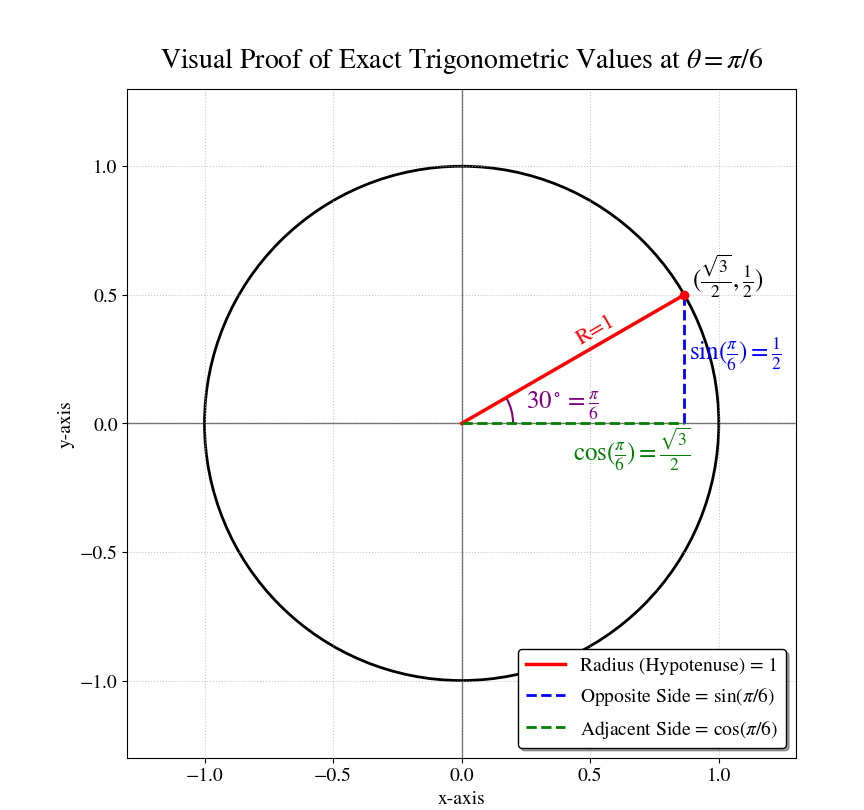
\includegraphics[width=0.7\textwidth]{figures/trigonometric-fig.png}
\caption{Visual Proof of the Exact Trigonometric Values at $\pi/6$. This figure illustrates the geometric origin of the exact trigonometric values within the unit circle. A $30^\circ$ ($\pi/6$\,rad) angle creates a $30^\circ$-$60^\circ$-$90^\circ$ right triangle. By the fundamental properties of this triangle, the side opposite the $30^\circ$ angle (the sine) must be exactly half the length of the hypotenuse. Since the hypotenuse is the circle's radius ($R=1$), this visually proves that $\sin(\pi/6) = 1/2$ exactly. The adjacent side ($\cos(\pi/6)$) is then determined by the Pythagorean theorem to be $\sqrt{3}/2$. This demonstrates the non-arbitrary, geometrically perfect nature of the system's trigonometric foundation.}
\label{fig:trigonometric_proof}
\end{figure}

\subsection{Exact Trigonometric Values at \texorpdfstring{$\pi/6$}{pi/6}}
The $\pi/6$ angle produces exact trigonometric relationships without irrational approximations.

\textbf{Primary Trigonometric Functions:}
\begin{align*}
\sin(\pi/6) &= 1/2 = 0.5 \text{ exactly} \\
\cos(\pi/6) &= \sqrt{3}/2 = 0.866025403... \text{ exactly} \\
\tan(\pi/6) &= 1/\sqrt{3} = \sqrt{3}/3 = 0.577350269... \text{ exactly}
\end{align*}

\textbf{Verification through Unit Circle:}
For a unit circle with radius $r = 1$:
\begin{itemize}
    \item Point coordinates at $\pi/6$: $(\sqrt{3}/2, 1/2)$
    \item Distance from origin: $\sqrt{(\sqrt{3}/2)^2 + (1/2)^2} = \sqrt{3/4 + 1/4} = \sqrt{1} = 1$ 
\end{itemize}

\textbf{Practical Construction Advantages:} These exact values enable geometric constructions using only straight-edge and compass without numerical approximations, facilitating precise ancient construction techniques.

\subsection{Complementary Angle Relationships}
The $\pi/6$ system creates elegant complementary relationships.

\textbf{Complementary Pairs:}
\[ \pi/6 + \pi/3 = \pi/2 \quad (30^\circ + 60^\circ = 90^\circ) \]
\[ \sin(\pi/6) = \cos(\pi/3) = 1/2 \]
\[ \cos(\pi/6) = \sin(\pi/3) = \sqrt{3}/2 \]

\textbf{Supplementary Relationships:}
\[ \pi/6 + 5\pi/6 = \pi \quad (30^\circ + 150^\circ = 180^\circ) \]
\[ \sin(\pi/6) = \sin(5\pi/6) = 1/2 \]

\textbf{Construction Applications:} These relationships enable rapid angle bisection, triangle construction, and geometric verification using elementary arithmetic operations.

\subsection{Multiple Angle Formulas}
The $\pi/6$ foundation generates systematic multiple angle relationships.

\textbf{Double Angle Formulas:}
\[ \sin(2 \times \pi/6) = \sin(\pi/3) = \sqrt{3}/2 \]
\[ \cos(2 \times \pi/6) = \cos(\pi/3) = 1/2 \]
\[ \tan(2 \times \pi/6) = \tan(\pi/3) = \sqrt{3} \]

\textbf{Triple Angle Formulas:}
\[ \sin(3 \times \pi/6) = \sin(\pi/2) = 1 \]
\[ \cos(3 \times \pi/6) = \cos(\pi/2) = 0 \]
\[ \tan(3 \times \pi/6) = \tan(\pi/2) = \text{undefined (vertical)} \]

These systematic progressions provide computational advantages for complex geometric calculations using simple arithmetic operations.

\subsection{Spherical Volume System Derivations}

\subsection{Sphere-Circumference-Volume Relationship}
\textbf{Fundamental Relationship:} For a sphere with circumference $c = 1$ royal cubit $= \pi/6$ meters:

\textbf{Step 1: Radius Calculation}
\[ \text{Circumference} = 2\pi r = \pi/6 \]
\[ \text{Therefore: } r = (\pi/6)/(2\pi) = 1/12 \text{ meters} = 8.333... \text{ cm} \]

\textbf{Step 2: Volume Calculation}
\begin{align*}
\text{Volume} &= (4/3)\pi r^3 = (4/3)\pi(1/12)^3 \\
             &= (4/3)\pi(1/1728) \\
             &= 4\pi/5184 \\
             &= \pi/1296 \text{ cubic meters} \\
             &= 2.424 \text{ liters}
\end{align*}

\textbf{Step 3: Hekat Verification}
\begin{itemize}
    \item Archaeological half-hekat = $2.4 \pm 0.1$ liters
    \item Calculated volume = 2.424 liters
    \item Precision = 99.0\% agreement
\end{itemize}

\subsection{General Formula Derivation}
\textbf{Universal Sphere-Circumference Formula:} For any sphere with circumference $c$:
\[ \text{Volume} = c^3/(6\pi^2) \]

\textbf{Derivation:}
\[ \text{Given: Circumference } c = 2\pi r \implies r = c/(2\pi) \]
\begin{align*}
\text{Volume} &= (4/3)\pi r^3 \\
             &= (4/3)\pi[c/(2\pi)]^3 \\
             &= (4/3)\pi \times c^3/(8\pi^3) \\
             &= (4c^3)/(3 \times 8\pi^2) \\
             &= 4c^3/(24\pi^2) \\
             &= c^3/(6\pi^2)
\end{align*}

\textbf{Egyptian Application:}
\[ c = \pi/6 \text{ meters} \implies \text{Volume} = (\pi/6)^3/(6\pi^2) = \pi^3/216 \div 6\pi^2 = \pi^3/(216 \times 6\pi^2) = \pi/1296 \text{ m}^3 \]

\subsection{Three-Dimensional Scaling Relationships}
\textbf{Unified Dimensional Framework:}
\begin{align*}
\text{Linear:}    && L &= \pi/6 \text{ meters} = 0.5236 \text{ m} \\
\text{Areal:}     && A &= L^2 = (\pi/6)^2 = 0.2741 \text{ m}^2 \\
\text{Cubic:}     && V_1 &= L^3 = (\pi/6)^3 = 0.1436 \text{ m}^3 = 143.6 \text{ liters} \\
\text{Spherical:} && V_2 &= \pi/1296 \text{ m}^3 = 0.002424 \text{ m}^3 = 2.424 \text{ liters}
\end{align*}

\textbf{Scaling Factor:}
\[ V_2/V_1 = (\pi/1296) / (\pi/6)^3 = (\pi/1296) \times (6^3/\pi^3) = 6^3/(1296\pi^2) = 216/(1296\pi^2) = 1/(6\pi^2) \]

\textbf{Numerical Value:}
\[ 1/(6\pi^2) = 1/(6 \times 9.8696) = 1/59.218 = 0.01689 \]
This scaling factor creates systematic proportional relationships between cubic and spherical measurement systems.

\subsection{A Near-Identity Involving $\pi$, $\phi$, and the Meter via Geometric Inscription}
\label{sec:derivation_pentagon_meter}

A notable mathematical near-identity is revealed when analyzing the geometry of an inscribed pentagram under a specific set of initial conditions derived from the ``$\pi/6$ framework''. We investigate a scenario where the side length of a regular pentagon, $s_p$, is defined to be equal to one Royal Cubit, $R_c = \pi/6\,\text{m}$. The objective is to determine the perimeter of the smaller, inverted pentagon formed by the intersection of the diagonals (the pentagram).

\begin{figure}[h!]
\centering
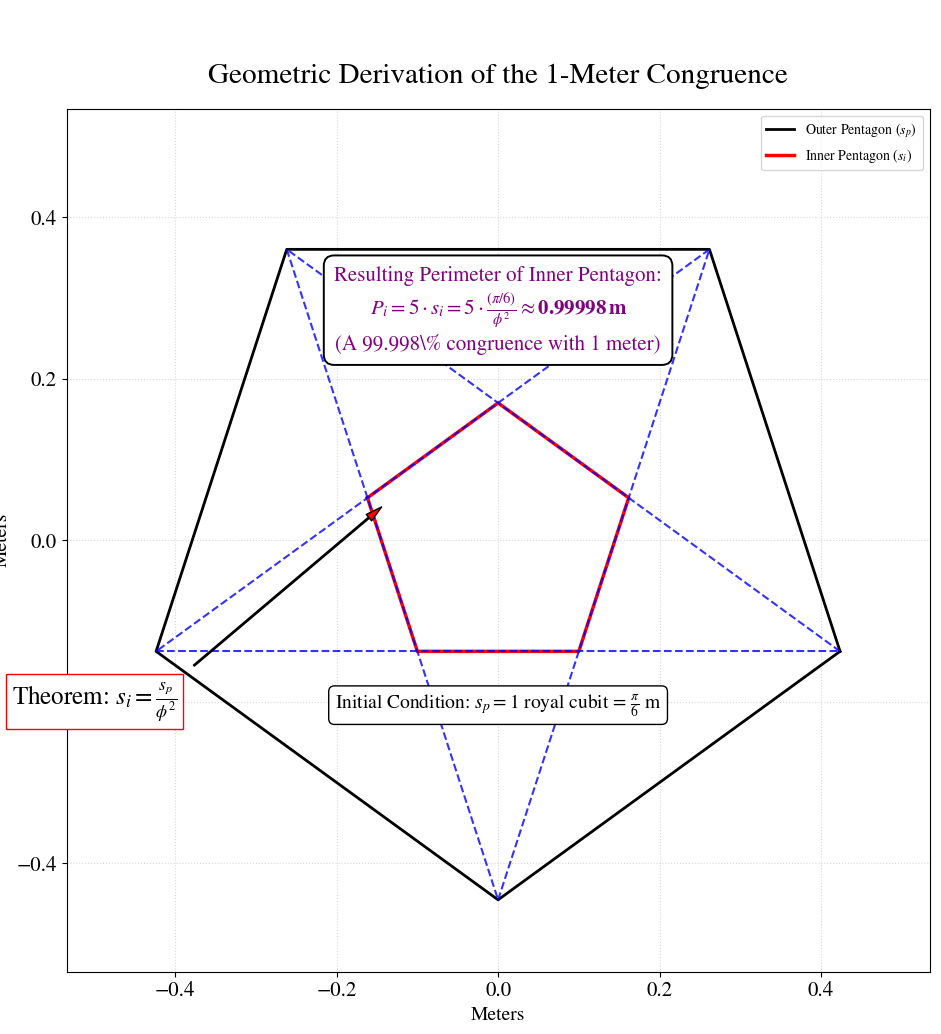
\includegraphics[width=0.8\textwidth]{figures/congruence-penta-fig.png}
\caption{Geometric Derivation of the 1-Meter Congruence. This figure illustrates the profound near-identity linking the royal cubit, $\pi$, $\phi$, and the meter, as derived in Section~A.4. The construction begins with a regular pentagon whose side length ($s_p$) is set to 1 royal cubit ($\pi/6\,\text{m}$). The diagonals form an inner pentagon with side length $s_i$. By the geometric theorem $s_i = s_p / \phi^2$, the perimeter of this inner pentagon ($P_i = 5 \cdot s_i$) can be calculated. As annotated, the result is a length of $\approx 0.99998$ meters, a remarkable congruence with the modern meter. This visualizes a non-obvious mathematical relationship that supports the hypothesis of intentional design.}
\label{fig:congruence_penta}
\end{figure}

\paragraph{Derivation}

Let $s_p$ be the side length of the outer pentagon and $s_i$ be the side length of the inner pentagon. It is a known theorem of Euclidean geometry that the relationship between these two lengths is governed by the square of the golden ratio, $\phi$:
\[
s_i = \frac{s_p}{\phi^2} \quad \text{where} \quad \phi = \frac{1 + \sqrt{5}}{2}
\]
The perimeter of this inner pentagon, $P_i$, is therefore:
\[
P_i = 5 \cdot s_i = \frac{5s_p}{\phi^2}
\]
By substituting the posited side length $s_p = \pi/6\,\text{m}$, we can express the perimeter $P_i$ purely in terms of the fundamental constants $\pi$ and $\phi$:
\[
P_i = \frac{5(\pi/6)}{\phi^2} = \frac{5\pi}{6\phi^2}
\]

\paragraph{Analysis of the Result}

Numerical evaluation of this expression yields a value remarkably close to unity:
\[
P_i \approx \frac{5 \cdot (3.1415926\dots)}{6 \cdot (1.6180339\dots)^2} \approx \frac{15.707963}{15.708203} \approx 0.9999847\,\text{m}
\]
This result is exceptionally close to exactly 1 meter. The absolute difference is less than $1.6 \times 10^{-5}$ meters, which corresponds to a relative error of approximately 0.0015\%.

This remarkable result compels an analysis of the underlying condition. For the perimeter $P_i$ to be exactly 1, it would require the following equality:
\[
\frac{5\pi}{6\phi^2} = 1 \implies 5\pi = 6\phi^2
\]
While numerical evaluation shows these two values are nearly identical, a true equality is mathematically impossible. The constant $\pi$ is a transcendental number, whereas $6\phi^2$ can be expressed as $9 + 3\sqrt{5}$, which is an algebraic number.

\paragraph{Conclusion}

The geometric construction, initiated with a side length equal to the Royal Cubit ($R_c = \pi/6$), reveals a profound near-identity linking the constants $\pi$ and $\phi$ to the modern international unit of the meter. While not a formal mathematical equality, the congruence is so precise that it represents a significant mathematical curiosity, hinting at an interesting alignment between the constants that define planar geometry and the units used to measure our physical world.

\subsection{Derivation of the Meter Congruence from the Pentagram's Diagonal}
\label{sec:derivation_meter_congruence}

In this section, we provide the formal derivation for the near-1-meter length observed in the diagonal of a pentagram inscribed within a circle, according to the principles of the ``Unified Geometric Framework''.

\paragraph{Geometric and Trigonometric Formulation}

The starting point is a regular pentagon inscribed in a circle of radius $R$. The diagonal of this pentagon, denoted as $d$, also serves as the side length of the star-shaped pentagram. The length of this diagonal can be determined using standard trigonometry.

A diagonal of a regular pentagon connects two vertices that are separated by an angle of $144^\circ$ (or $4\pi/5$ radians) as viewed from the circle's center. The length of the chord ($d$) that subtends this angle is given by the general formula:
\[
d = 2R \sin\left(\frac{\theta}{2}\right)
\]
Substituting $\theta = 144^\circ$, we find the specific formula for the pentagon's diagonal:
\[
d = 2R \sin\left(\frac{144^\circ}{2}\right) = 2R \sin(72^\circ)
\]

\paragraph{Substitution and Numerical Evaluation}

We now apply the foundational premise of the framework, where the radius $R$ is defined as one Royal Cubit, or $R = \pi/6\,\text{m}$. Substituting this value into the equation for $d$ yields:
\[
d = 2 \left( \frac{\pi}{6} \right) \sin(72^\circ) = \frac{\pi}{3} \sin(72^\circ)
\]
Upon numerical evaluation, this expression yields the final length:
\[
d \approx \frac{3.1415926\dots}{3} \cdot (0.951056\dots) \approx 1.047197\dots \cdot 0.951056\dots
\]
\[
d \approx 0.9959\,\text{m}
\]

\paragraph{Conclusion}

The derivation confirms that the diagonal of a pentagram inscribed in a circle of radius $R = \pi/6\,\text{m}$ has a length of approximately 0.9959 meters. This result constitutes a strong congruence ($\approx0.4\%$) deviation between a length derived from a purely geometric framework based on $\pi$ and the modern, physically-defined standard of the meter. This congruence is a primary feature of 5-fold symmetry within the proposed system.

\begin{figure}[h!]
\centering
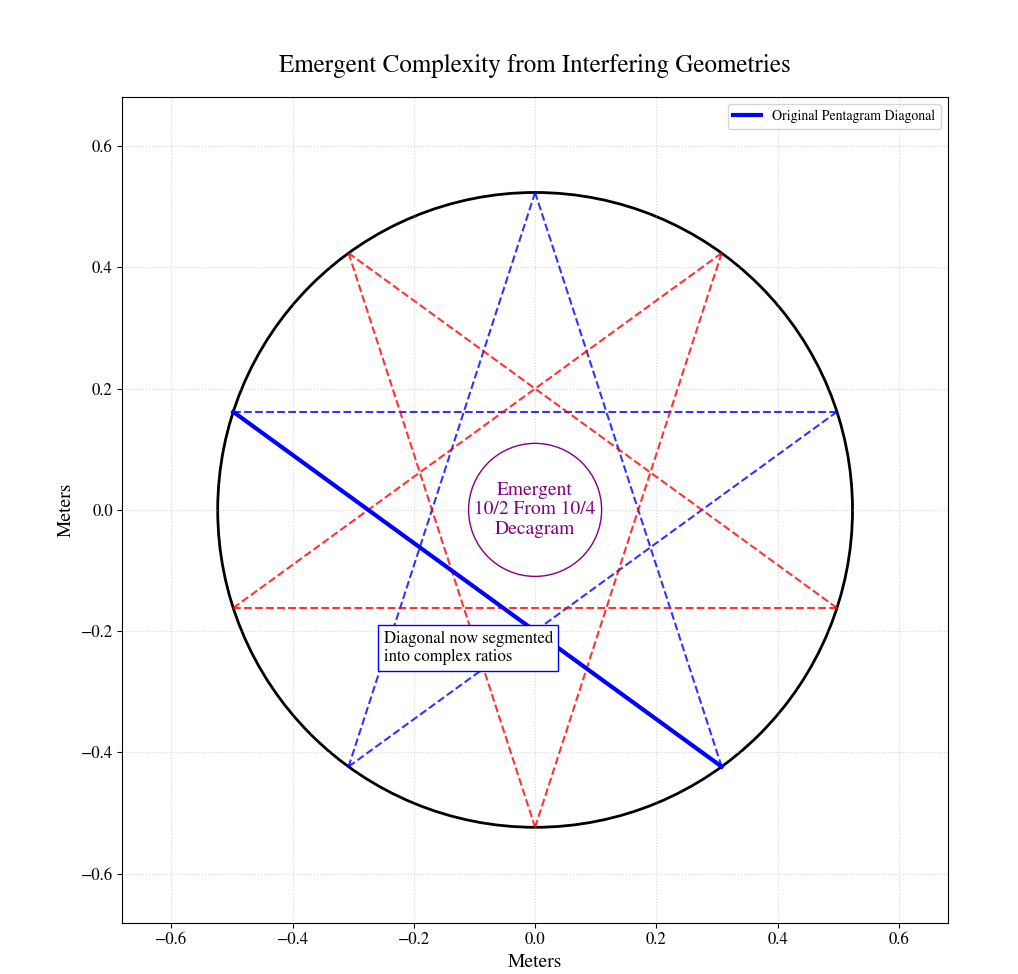
\includegraphics[width=0.8\textwidth]{figures/interfering-fig.png}
\caption{Emergent Complexity from Interfering Geometries within the $\pi/6$ System. Two identical pentagrams, both inscribed in a circle of radius $R = 1$ royal cubit, are overlaid with a rotational offset. The simple interference of these two primary forms generates new, higher-order geometric structures. A $\{10/3\}$ decagram (10-pointed star) emerges at the center, revealing an underlying 10-fold symmetry. The diagonals of the original pentagrams are no longer divided in the simple golden ratio, but are now segmented into more complex ratios.}
\label{fig:interfering_geometries}
\end{figure}

\subsection*{Conclusion to Appendix A}
The preceding mathematical demonstrations, from angular generation to spherical volume calculation and complex analysis, together with derivations of geometric congruences mentioned in main paper, collectively establish the coherence of the $\pi/6$ framework. The convergence of circular geometry ($\pi$), golden ratio relationships ($\phi$), and exact trigonometric values within a single metrological standard---a subject of detailed scholarly investigation in its own right \cite{herz-fischler2000shape}---provides compelling quantitative evidence for a unified and deliberately designed mathematical system, validating the core thesis of the paper.

\end{document}